\chapter{The way of the program}

The goal of this book is to teach you to think like a computer scientist.
This way of thinking combines some of the best features of mathematics, engineering, and natural science.
Like mathematicians, computer scientists use formal languages to denote ideas (specifically computations).
Like engineers, they design things, assembling components into systems and evaluating trade-offs among alternatives.
And like scientists, they observe the behavior of complex systems, form hypotheses, and test predictions.

\index{problem-solving}

The single most important skill for a computer scientist is {\bf problem-solving}.
It involves the ability to formulate problems, think creatively about solutions, and express a solution clearly and accurately.
As it turns out, the process of learning to program is an excellent opportunity to develop problem-solving skills.
That's why this chapter is called, ``The way of the program.''

On one level you will be learning to program, a useful skill by itself.
But on another level you will use programming as a means to an end.
As we go along, that end will become clearer.
Learning how to think in terms of computation is much more valuable than simply learning how to write code.

\section{What is programming?}

\index{program}

A {\bf program} is essentially a sequence of instructions that specifies how to perform a computation.
%\footnote{This definition does not apply to all programming languages; for alternatives, see \url{http://en.wikipedia.org/wiki/Declarative_programming}.}
The computation might be something mathematical, like solving a system of equations or finding the roots of a polynomial.
It can also be a symbolic computation, like searching and replacing text in a document or (strangely enough) compiling a program.
The details look different in different languages, but a few basic instructions appear in just about every language.

\begin{description}
\item[input:] Get data from the keyboard, a file, a sensor, or some other device.
\item[output:] Display data on the screen or send data to a file or other device.
\item[math:] Perform basic mathematical operations like addition and division.
\item[decisions:] Check for certain conditions and execute the appropriate code.
\item[repetition:] Perform some action repeatedly, usually with some variation.
\end{description}

\index{programming}

Believe it or not, that's pretty much all there is to it.
Every program you've ever used, no matter how complicated, is made up of instructions that look much like these.
So you can think of {\bf programming} as the process of breaking down a large, complex task into smaller and smaller subtasks.
The process continues until the subtasks are simple enough to be performed with the basic instructions provided by computer hardware.

\section{What is computer science?}

One of the most interesting aspects of writing programs is deciding how to solve a particular problem, especially when there are multiple solutions.
For example, there are numerous ways to sort a list of names or numbers, each with its own advantages (see e.g., \url{http://www.sorting-algorithms.com/}).
In order to determine which way is best for a given situation, we need techniques for describing and analyzing solutions formally.
That is where computer science comes in.

\index{computer science}
\index{algorithm}

Put simply, {\bf computer science} is the science of algorithms, including their discovery and analysis.
An {\bf algorithm} is a sequence of steps that specify exactly how to solve a problem.
Some algorithms are better than others in terms of low long they take or how much memory they use.
As you learn to develop algorithms for problems you haven't solved before, you also learn to think like a computer scientist.
It's much more fun to discover new algorithms than to write the code for solutions that other people came up with!

\index{bug}
\index{debugging}

Designing algorithms and writing code is difficult and error-prone.
One of the most important problem-solving skills you will learn is how to debug your programs.
For historical reasons, programming errors are called {\bf bugs}, and the process of tracking them down and correcting them is called {\bf debugging}.
In the old days, computer scientists had to deal with real bugs flying into their systems.
You probably won't have that problem, but you will need to think creatively when unexpected errors happen.

\begin{figure}[h!]
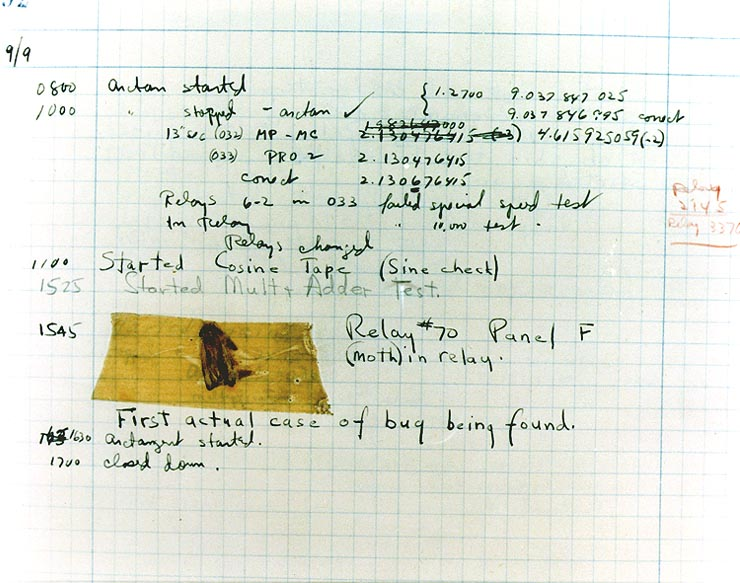
\includegraphics[height=2.2in]{firstbug.jpg}
\caption{The first computer bug, taped to Grace Hopper's log book in 1947.
\\ She discovered the moth in an electromagnetic relay of the Mark II.}
\end{figure}

Although it can be frustrating, debugging is one of the most intellectually rich, challenging, and interesting parts of computer programming.
In some ways, debugging is like detective work.
You are confronted with clues, and you have to infer the processes and events that led to the results you see.
Thinking about how to correct programs and improve their performance sometimes even leads to the discovery of new algorithms.

\section{Introduction to Java}

\index{high-level language}
\index{language!high-level}

The programming language you will be learning is Java, which is relatively new (Sun released the first version in May 1995).
Java is an example of a {\bf high-level language}.
Other high-level languages you may have heard of include C, C++, C\#, Objective-C, Perl, PHP, Python, Ruby, and Visual Basic.

\index{low-level language}
\index{language!low-level}

There are also {\bf low-level languages}, sometimes referred to as ``machine languages'' or ``assembly languages.''
Loosely speaking, computers can only run programs written in low-level languages.
So programs written in a high-level language have to be translated before they can run.
This translation takes some time, which is a small disadvantage of high-level languages.

\index{portable}

But the advantages of high-level languages are enormous.
First, it is {\em much} easier to program in a high-level language.
Programs take less time to write, are shorter and easier to read, and are more likely to be correct.
Second, high-level languages are {\bf portable}, meaning that they can run on different kinds of computers with few or no modifications.
Low-level programs can only run on one kind of computer, and have to be rewritten to run on another.
Due to the advantages, almost all programs are written in high-level languages.
Low-level languages are only used for a few special applications (e.g., device drivers).

\index{interpreter}

Two kinds of programs translate high-level languages into low-level languages: interpreters and compilers.
An {\bf interpreter} reads a high-level program and executes it, meaning that it does what the program says.
It processes the program a little at a time, alternately reading lines and performing computations on the fly.
% Figure 1.1 shows the structure of an interpreter.

\begin{center}
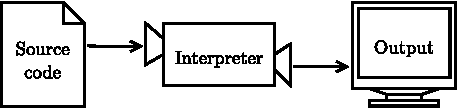
\includegraphics{interpreter.pdf}
\end{center}

\index{compiler}
\index{source code}
\index{object code}
\index{executable}

A {\bf compiler} reads the entire program and translates it completely before the program starts running.
In this context, the high-level program is called the {\bf source code}, and the translated program is called the {\bf object code} or the {\bf executable}.
Once a program is compiled, you can execute it repeatedly without further translation.
As a result, compiled programs often run faster than interpreted programs.
% Figure 1.2 shows the structure of a compiler.

\index{byte code}

Java is {\em both} compiled and interpreted.
Instead of translating programs directly into machine language, the Java compiler generates {\bf byte code}.
Similar to machine language, byte code is easy (and fast) to interpret.
But it is also portable, like a high-level language.
Thus it is possible to compile a Java program on one machine, transfer the byte code to another machine, and then execute (interpret) the byte code on the other machine.
This ability is an advantage of Java over many other high-level languages.

\begin{center}
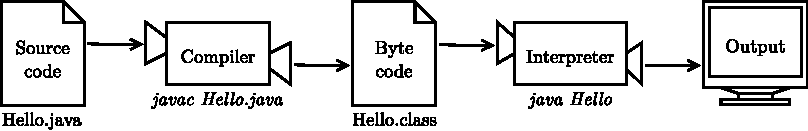
\includegraphics{compiler.pdf}
\end{center}

Although this process may seem complicated, in most program development environments these steps are automated for you.
Usually you will only have to write a program and press a button or type a single command to compile and run it.
On the other hand, it is important to know what steps are happening in the background, so if something goes wrong you can figure out what it is.

\section{Formal languages}

\index{natural language}
\index{language!natural}

Learning a programming language is very different from learning a {\bf natural language} such as English, Spanish, French, or German.
The languages that people speak evolved naturally over time.
They were not designed by people, although we try to impose order on them for practical reasons.

\index{formal language}
\index{language!formal}

In contrast, {\bf formal languages} are designed by people for specific applications.
For example, the notation that mathematicians use is a formal language that is particularly good at denoting relationships among numbers and symbols.
Chemists use a formal language to represent the chemical structure of molecules.
And most importantly:

\index{programming language}
\index{language!programming}

\begin{quote}
{\bf Programming languages are formal languages that have been designed to express computations.}
\end{quote}

\index{syntax}
\index{semantics}

Formal languages have strict rules about both the {\bf syntax} (structure) and the {\bf semantics} (meaning) of statements.
For example, $3 + 3 = 6$ is a syntactically correct mathematical statement, but $3\ + = 3\ \$\ 6$ is not.
$1 + 2 = 4$ uses correct syntax, but is semantically incorrect.
$H_2O$ is a syntactically correct chemical formula, but $_2Zz$ is not.

\subsection{Tokens and grammar}

\index{token}

Syntax rules come in two flavors, pertaining to tokens and grammar.
{\bf Tokens} are the basic elements of the language, like words, numbers, and chemical elements.
One of the problems with $3\ + = 3\ \$\ 6$ is that $\$$ is not a legal token in mathematics.
Similarly, $_2Zz$ is not legal because there is no element with the abbreviation $Zz$.

\index{grammar}

The second type of syntax rule pertains to the {\bf grammar} of the language, or the way that individual tokens can be arranged.
The statement $3\ + = 3$ is structurally illegal, even though $+$ and $=$ are legal tokens, because you can't have one right after the other.
Similarly, in a chemical formula the subscript comes after the element name, not before.

\index{parse}

When you read a sentence in English or a statement in a formal language, you have to figure out the structure of the sentence (although in a natural language you do this unconsciously).
This process is called {\bf parsing}.
For example, when you hear the statement ``the penny dropped,'' you understand that the penny is the subject and dropped is the predicate.
After you have parsed the statement, you can begin to figure out what it means.
%Assuming that you know what a penny is and what it means to drop, you will understand the general implication of this statement.

Although formal and natural languages have features in common---tokens, grammar, and meaning---there are some differences.

\begin{description}

\term{ambiguity}
Natural languages are full of ambiguity, which people deal with by using contextual clues and other information.
Formal languages are designed to be nearly or completely unambiguous, which means that any statement has exactly one meaning, regardless of context.

\term{redundancy}
In order to make up for ambiguity and reduce misunderstandings, natural languages employ lots of redundancy.
As a result, they are often verbose.
Formal languages are less redundant and more concise.

\term{literalness}
Natural languages are full of idiom and metaphor.
When someone says ``the penny dropped'' there is no penny and nothing dropping.
This idiom means that someone finally realized something after a period of confusion.
In contrast, formal languages mean exactly what they say.

\end{description}

\subsection{Reading source code}

People who grow up speaking a natural language---that is, everyone---often have a hard time adjusting to formal languages.
In some ways, the difference between natural and formal language is like the difference between poetry and prose, but more so.

\begin{description}

\term{poetry}
Words are used for their sounds as well as for their meaning, and the whole poem together creates an effect or emotional response.
Ambiguity is not only common but often deliberate.

\term{prose}
The literal meaning of words is more important, and the structure contributes more meaning.
Prose is more amenable to analysis than poetry but still often ambiguous.

\term{program}
The meaning of a computer program is unambiguous and literal, and can be understood entirely by analysis of the tokens and grammar.

\end{description}

Here are some suggestions for reading programs (and other formal languages).
First, remember that formal languages are much more dense than natural languages, so it takes longer to read them.
Second, the structure is very important, so it is not always a good idea to read from top to bottom, left to right.
Over time you will learn to parse the program in your head, identifying the tokens and interpreting the structure.
Finally, the details matter.
Small errors in spelling and punctuation, which you can get away with in natural languages, can make a big difference in a formal language.

\section{The hello world program}
\label{hello}

\index{hello world}

Traditionally, the first program you write when learning a new programming language is called the hello world program.
All it does is display the words ``Hello, World!''
In Java, it looks like this:

\begin{code}
public class Hello {

    public static void main(String[] args) {
        // generate some simple output
        System.out.println("Hello, World!");
    }

}
\end{code}

\index{public}
\index{static}

Unfortunately for Java, even this simple example requires language features that are difficult to explain to beginners.
But it provides a preview of topics that we will see in detail later on.
The word \java{public} means the code can be accessed from other source files.
The word \java{static} means that memory is allocated for the program in advance.
We will discuss \java{void}, \java{String}, and \java{args} in the next chapter.
For now, let's focus on the overall structure.

\index{class!definition}
\index{method!definition}

Java programs are made up of {\bf class} and {\bf method} definitions, which generally have the form:

\begin{code}
public class CLASSNAME {

    METHOD {
        STATEMENTS
    }

    METHOD {
        STATEMENTS
    }

}
\end{code}

\index{class!name}

Here {\tt CLASSNAME} indicates the name chosen by the programmer.
Java requires the class name to match the source file name.
In the hello world example, the file name must be Hello.java because the class name is \java{Hello}.

\index{statement}
\index{main}

Classes define a program's methods, or named sequences of {\bf statements}.
The \java{Hello} class has only one method.
The name \java{main} is special; it marks the place in the class where execution begins.
When the program runs, it starts at the first statement in \java{main} and ends when it finishes the last statement.

\index{braces}
\index{squiggly braces}

Java uses squiggly braces (\{ and \}) to group things together.
In Hello.java, the outermost squiggly braces (lines 1 and 8) contain the class definition, and the inner braces (lines 3 and 6) contain the definition of \java{main} method.

\index{println}
\index{statement!print}

The main method can have any number of statements, but the \java{Hello} example has only one.
It is a {\bf print statement}, meaning that it displays a message on the screen.
Confusingly, print can mean both ``display something on the screen'' and ``send something to the printer.''
%I won't say much about sending things to the printer;
In this book, we'll do all our printing on the screen.
The print statement ends with a semicolon ({\tt ;}).

%\index{library}
%
%{\tt System.out.println} is a method provided by one of Java's standard libraries.
%A {\bf library} is a collection of class and method definitions that you can use in your programs.

\index{comment}
\index{statement!comment}

Line 4 contains a {\bf comment}, or a bit of English text that explains the code that follows.
When the compiler sees \java{//}, it ignores everything from there until the end of the line.
You should {\em always write comments} before every major block of code so that other programmers (including your future self) can understand what you meant to do.

\subsection{Getting started with DrJava}

\index{JDK}

In order to compile Java programs on your own computer, you will need to install the Java Development Kit (JDK).
This free software by Oracle includes tools for developing, debugging, and monitoring Java applications.
All the examples in this book were developed and tested using Java SE Version 7.
Later versions of Java are generally backward compatible, so feel free to install the latest and greatest release.

\index{DrJava}

We will use DrJava as the primary development environment throughout the book.
One of the most distinctive features of DrJava is the Interactions Pane at the bottom of the window.
It offers both beginning students and more experienced programmers the ability to try out code quickly, without having to write a class definition and save/compile/run the program.
Refer to the DrJava documentation (\url{http://drjava.org/docs/quickstart/}) for more details.

\begin{figure}[h!]
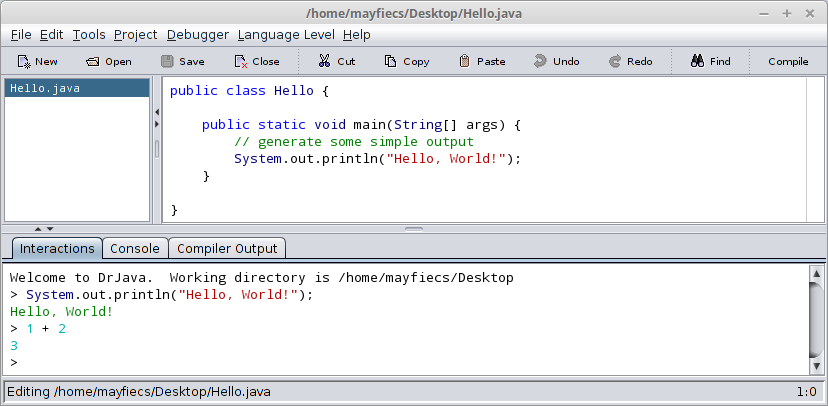
\includegraphics[width=\textwidth]{drjava-hello.png}
\caption{Screenshot of DrJava editing the hello world program.}
\end{figure}

Step-by-step instructions for installing the JDK and configuring DrJava are available on this book's website: \url{http://thinkjava.org/}

\section{Reading error messages}

\index{error!message}

As you begin writing your own programs, you will encounter various error messages.
Three kinds of errors can occur in a program: syntax errors, runtime errors, and semantic errors.
It is useful to distinguish between them in order to track them down more quickly.
Regardless of what type of error occurs, always remember to {\em read and think about the error messages carefully}.
They will usually point you in the right direction to fix your program.

\subsection{Syntax errors}

\index{syntax error}
\index{error!syntax}

The compiler can only translate a program if the syntax is correct; otherwise, the compilation fails and displays an error message.
For example, parentheses have to come in matching pairs.
So (1 + 2) is legal, but 8) is a {\bf syntax error}.

In English, readers can tolerate most syntax errors, which is why we can read the poetry of e.\ e.\ cummings without spewing error messages.
Java is not so forgiving, and there are more syntax rules in Java than there are in English.
If there is a single syntax error anywhere in your program, the compiler will display an error message and quit, and you will not be able to run your program.

\begin{figure}[h!]
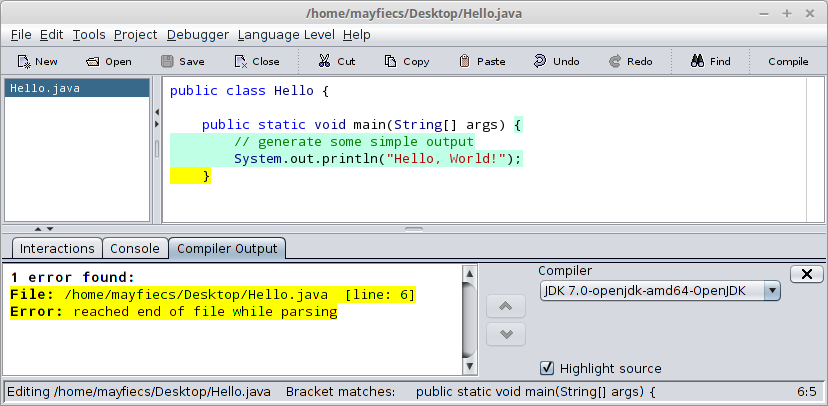
\includegraphics[width=\textwidth]{syntax-error.png}
\caption{A syntax error caused by a missing brace.}
\end{figure}

To make matters worse, the error messages you get from the compiler are often not very helpful.
For example, removing the closing brace on line 8 of the hello world program results in ``Error: reached end of file while parsing.''
The compiler also reports that the problem was found on line 6, which in this case is not at fault.
Since line 8 was deleted, the compiler had no other choice.

During the first few weeks of your programming career, you will probably spend a lot of time tracking down syntax errors.
But as you gain experience, you will make fewer errors and find them more quickly.

\subsection{Runtime errors}

\index{runtime error}
\index{error!runtime}
\index{type-safe}
\index{language!type-safe}

The second type of error is a runtime error, so called because it does not appear until after the program has started running.
In Java, these errors occur when the interpreter is executing the byte code and something goes wrong.
Java is designed to be a {\bf type-safe} language, which means that the compiler can detect many potential errors cased by common programming mistakes.
Runtime errors are rare in the simple programs you will see in the first few chapters, so it might be a while before you encounter them.

\index{exception}

These errors are also called {\bf exceptions} because they usually indicate that something exceptional (and bad) has happened.
In most environments they appear as windows or dialog boxes that contain information about what happened and what the program was doing when it happened.
For example, if you accidentally divide by zero you will get an \java{ArithmeticException}:

\begin{small}
\begin{stdout}
Exception in thread "main" java.lang.ArithmeticException: / by zero
    at Hello.main(Hello.java:5)
\end{stdout}
\end{small}

This information is useful for debugging.
The first line gives a brief description of the error (/ by zero).
The subsequent lines report the class and method names (Hello.main), along with the file names and line numbers of where the error occurred (Hello.java:5).
Keep in mind that the exact line where the program crashed may not be the line that needs to be fixed.

\subsection{Semantic errors}

\index{logic error}
\index{error!logic}

The third type of error is the semantic or {\bf logic error}.
If there is an error in your program's logic, it will compile and run successfully in the sense that the computer will not generate any error messages.
But it will not do the right thing.
It will do something else.
Specifically, it will do what you told it to do.
Here is an example of a semantic error in the hello world program:

\begin{code}
public class Hello {

    public static void main(String[] args) {
        System.out.println("Goodbye, world.");
    }

}
\end{code}

Note that this program compiles and runs just fine.
The problem is that the main method is not the program we intended.
The meaning of the program (its semantics) is wrong, because it says goodbye instead of hello. In addition, world is not capitalized, and it ends with a period instead of an exclamation point.
Identifying semantic errors can be tricky because it requires you to challenge your assumptions about the code.
You will need to work backward by looking at the output of the program, and try to figure out what it is doing.

\section{Working through examples}

It is a good idea to read this book in front of a computer so you can try out the examples as you go.
You can run many of the examples directly in DrJava's Interactions Pane, but if you put the code in a source file, it will be easier to try out variations.

Whenever you are experimenting with a new feature, you should also try to make mistakes.
For example, in the hello world program, what happens if you leave out one of the quotation marks?
What if you leave out both?
What if you spell \java{println} wrong?
This kind of experiment helps you remember what you read.
It also helps with debugging, because you get to know what the error messages mean.
It is better to make mistakes now and on purpose than later on and accidentally.

\index{experimental debugging}
\index{debugging!experimental}

\index{Holmes, Sherlock}
\index{Doyle, Arthur Conan}

Debugging is like an experimental science.
Once you have an idea about what is going wrong, you modify your program and try again.
If your hypothesis was correct, then you can predict the result of the modification, and you take a step closer to a working program.
If your hypothesis was wrong, you have to come up with a new one.
As Sherlock Holmes pointed out, ``When you have eliminated the impossible, whatever remains, however improbable, must be the truth.''
(A.~Conan Doyle, {\em The Sign of Four}.)

Programming and debugging should go hand in hand.
Don't just write a bunch of code and then perform trial and error debugging until it all works.
Instead, start with a program that does {\em something} and make small modifications, debugging them as you go, until the program does what you want.
That way you will always have a working program, and it will be easier to isolate errors.

\index{Linux}
\index{Torvalds, Linux}
\index{Greenfield, Larry}

A great example of this principle is the Linux operating system, which contains millions of lines of code.
It started out as a simple program Linus Torvalds used to explore the Intel 80386 chip.
According to Larry Greenfield, ``One of Linus's earlier projects was a program that would switch between printing AAAA and BBBB.
This later evolved to Linux.'' ({\em The Linux Users' Guide})

%Later chapters will make more suggestions about debugging and other programming practices.

Finally, programming sometimes brings out strong emotions.
If you are struggling with a difficult bug, you might feel angry, despondent, or embarrassed.
Remember that you are not alone, and most if not all programmers have had similar experiences.
Don't hesitate to reach out to a friend and ask questions!

%\index{emotional debugging}
%\index{debugging!emotional response}

%There is evidence that people naturally respond to computers as if they were people.
%When they work well, we think of them as teammates, and when they are obstinate or rude, we respond to them the same way we respond to rude, obstinate people.
%(Reeves and Nass, {\it The Media Equation: How People Treat Computers, Television, and New Media Like Real People and Places})

%Preparing for these reactions might help you deal with them.
%One approach is to think of the computer as an employee with certain strengths, like speed and precision, and particular weaknesses, like lack of empathy and inability to grasp the big picture.

%Your job is to be a good manager: find ways to take advantage of the strengths and mitigate the weaknesses.
%And find ways to use your emotions to engage with the problem, without letting your reactions interfere with your ability to work effectively.

%Learning to debug can be frustrating, but it is a valuable skill that is useful for many activities beyond programming.
%At the end of each chapter there is a debugging section, like this one, with my thoughts about debugging.
%I hope they help!
